\subsection{BRACS}

El conjunto de datos BReAst Carcinoma Subtyping (BRACS), presentado en \cite{brancati2021bracs}, contiene imágenes teñidas con Hematoxilina y Eosina (H\&E), divididas en 547 Whole-Slide-Images (WSIs), 4539 Regiones de Interes (ROIs) extraidas de las WSIs. Cada WSI, y sus respectivas ROIs, están anotadas por el consenso de tres patólogos certificados en diferentes categorías de lesiones. Específicamente, BRACS incluye tres tipos de lesiones: benginas, malignas y atípicas, que a su vez se subdividen en un total de siete categorías.

Las WSI están almacenadas en formato .svs como una pirámide multi-resolución, donde la máxima resolución puede exceder fácilmente los 1000 $\times$ 1000 píxeles. Por otro lado, las ROI corresponde a una región con un aumento del 40$\times$ y su resolución puede exceder de los 4000$\times$4000 píxeles.

Ambos grupos de imágenes tienen el mismo tipo de agrupación, en el que las imágenes se separan en tres grandes grupos, BT -tumores benignos-, AT -tumores atípicos- y MT --tumores malignos-. 

El grupo BT contiene muestras de los tipos N, para muestra normal, PB para las muestras patológicamente Benignas, y UDH para muestras con Hiperplasia Ductal Usual.

El grupo AT se subdivide, a su vez, dos grupos. Por un lado el grupo FEA para la Atipia Epitelial Plana (\textit{Flat Epithelial Atypia}) y ADH para la Hiperplasia Ductal Atípica (\textit{Atypical Ductal Hyperplasia}).

Por último, el grupo MT se divide en dos subconjuntos, que incluyen muestras anotadas como Carcinoma Ductal in Situ (DCIS,  \textit{Ductal Carcinoma in Situ}), y Carcinoma Invasivo (IC, \textit{Invasive Carcinoma}).

% \begin{figure}
%     \centering
%     \includegraphics[width=\textwidth]{tex/latex/tfgetsinf/3.Datasets/img/BRACS_Diagram.png}
%     \caption{Organización de grupos del conjunto de datos BRACS}
%     \label{fig:BRACS_Diagram_B}
% \end{figure}


\begin{figure}[h]
\centering
    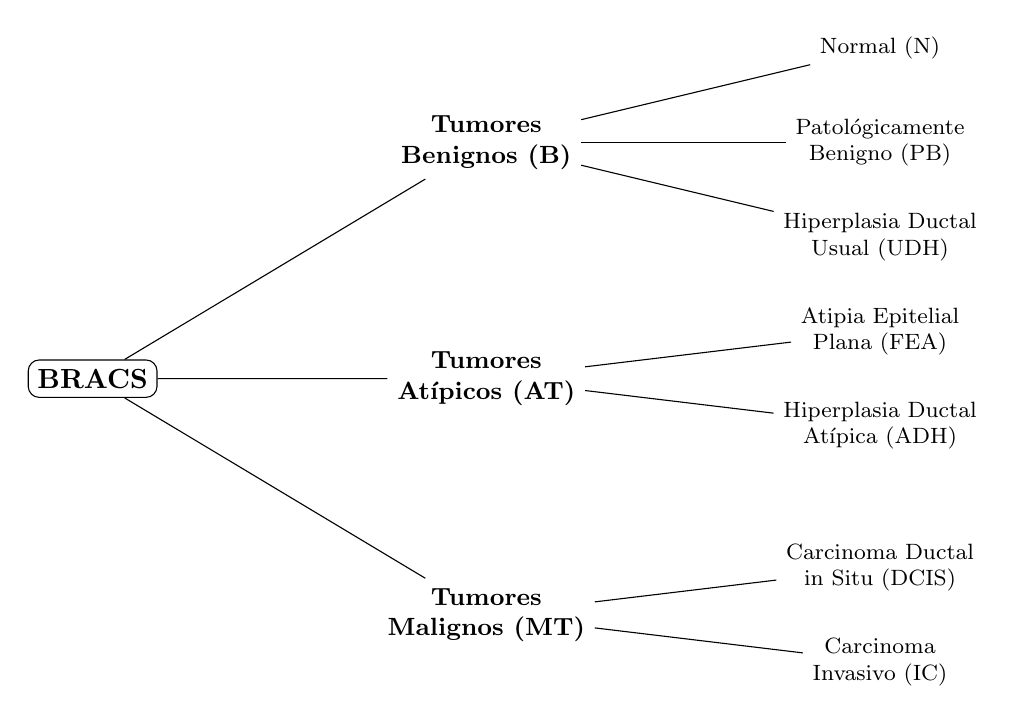
\begin{tikzpicture}[grow=right, level distance=5cm,
    level 1/.style={sibling distance=3cm},
    level 2/.style={sibling distance=1.2cm}]
    \node [rectangle, draw, rounded corners, font=\bfseries] {BRACS}
      child {node[font=\bfseries\small, align=center] {Tumores\\Malignos (MT)}
        child {node[font=\footnotesize, align=center] {Carcinoma\\Invasivo (IC)}}
        child {node[font=\footnotesize, align=center] {Carcinoma Ductal\\in Situ (DCIS)}}}
      child {node[font=\bfseries\small, align=center] {Tumores\\Atípicos (AT)}
        child {node[font=\footnotesize, align=center] {Hiperplasia Ductal\\Atípica (ADH)}}
        child {node[font=\footnotesize, align=center] {Atipia Epitelial\\Plana (FEA)}}}
      child {node[font=\bfseries\small, align=center] {Tumores\\Benignos (B)}
        child {node[font=\footnotesize, align=center] {Hiperplasia Ductal\\Usual (UDH)}}
        child {node[font=\footnotesize, align=center] {Patológicamente\\Benigno (PB)}}
        child {node[font=\footnotesize, align=center] {Normal (N)}}};
    \end{tikzpicture}
    \caption{Organización de grupos del conjunto de datos BRACS}
    \label{fig:BRACS_Diagram}
\end{figure}


\begin{table}[!ht]
    \centering
    \resizebox{\textwidth}{!}{
        \begin{tabular}{|l|l|l|l|l|l|l|l|}
        \hline
                   & \multicolumn{3}{|l|}{\textbf{Group\_BT}}  & \multicolumn{2}{|l|}{\textbf{Group\_AT}} & \multicolumn{2}{|l|}{\textbf{Group\_MT}} \\ \hline
                   & Type\_N & Type\_PB & Type\_UDH & Type\_FEA     & Type\_ADH     & Type\_DCIS     & Type\_IC     \\ \hline
        \textbf{Training}   & 27      & 120      & 56        & 24            & 28            & 40             & 100          \\ \hline
        \textbf{Validation} & 10      & 11       & 9         & 6             & 8             & 9              & 12           \\ \hline
        \textbf{Testing}    & 7       & 16       & 9         & 11            & 12            & 12             & 20           \\ \hline
        \end{tabular}
    }
    \caption{Estructura de imágenes WSI en el set de datos BRACS}
    \label{tab:BRACS_WSI}
\end{table}


\begin{table}[!ht]
    \centering
    \resizebox{\textwidth}{!}{
        \begin{tabular}{|l|l|l|l|l|l|l|l|}
        \hline
                   & \multicolumn{3}{|l|}{\textbf{Group\_BT}}  & \multicolumn{2}{|l|}{\textbf{Group\_AT}} & \multicolumn{2}{|l|}{\textbf{Group\_MT}} \\ \hline
                   & Type\_N & Type\_PB & Type\_UDH & Type\_FEA     & Type\_ADH     & Type\_DCIS     & Type\_IC     \\ \hline
        \textbf{Training}   & 357      & 714      & 389        & 624            & 387            & 665             & 521          \\ \hline
        \textbf{Validation} & 46      & 43       & 46         & 49             & 41             & 40              & 47           \\ \hline
        \textbf{Testing}    & 81       & 79       & 82         & 83            & 79            & 85             & 81           \\ \hline
        \end{tabular}
    }
    \caption{Estructura de imágenes ROI en el set de datos BRACS}
    \label{tab:BRACS_ROI}
\end{table}
